\documentclass[border=3pt]{standalone}
\usepackage{tikz}
\usetikzlibrary{arrows.meta,positioning}
\usepackage{amsmath}
\usepackage{xcolor}
\begin{document}
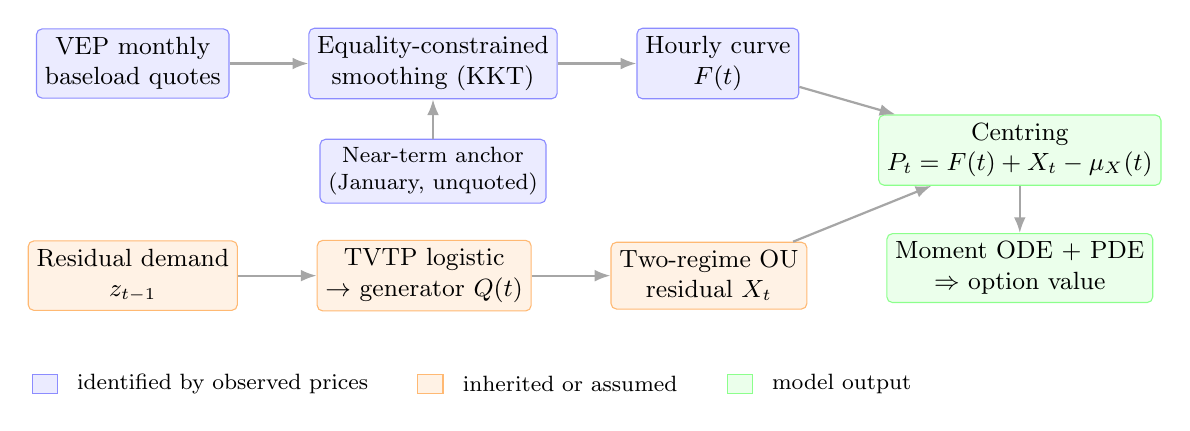
\begin{tikzpicture}[
  node distance=6mm,
  box/.style={draw,rounded corners=2pt,align=center,font=\small,
              minimum height=8mm,inner sep=3pt},
  mkt/.style={box,fill=blue!8,draw=blue!45},
  hist/.style={box,fill=orange!10,draw=orange!55},
  res/.style={box,fill=green!8,draw=green!45},
  arr/.style={-{Latex[length=2mm]},thick,draw=gray!70}
]
% market path
\node[mkt] (quotes) {VEP monthly\\baseload quotes};
\node[mkt,right=10mm of quotes] (qp) {Equality-constrained\\smoothing (KKT)};
\node[mkt,right=10mm of qp] (curve) {Hourly curve\\$F(t)$};
\node[mkt,below=5mm of qp,font=\footnotesize] (anchor) {Near-term anchor\\(January, unquoted)};

% historical path
\node[hist,below=18mm of quotes] (rd) {Residual demand\\$z_{t-1}$};
\node[hist,right=10mm of rd] (tvtp) {TVTP logistic\\$\to$ generator $Q(t)$};
\node[hist,right=10mm of tvtp] (ou) {Two-regime OU\\residual $X_t$};

% join
\node[res,right=10mm of curve,yshift=-11mm] (centre)
      {Centring\\$P_t=F(t)+X_t-\mu_X(t)$};
\node[res,below=6mm of centre] (price) {Moment ODE $+$ PDE\\$\Rightarrow$ option value};

\draw[arr] (quotes) -- (qp);
\draw[arr] (qp) -- (curve);
\draw[arr] (anchor) -- (qp);
\draw[arr] (rd) -- (tvtp);
\draw[arr] (tvtp) -- (ou);
\draw[arr] (curve) -- (centre);
\draw[arr] (ou) -- (centre);
\draw[arr] (centre) -- (price);

% legend
\node[below=9mm of rd.south west,anchor=north west,inner sep=0pt] (leg) {};
\node[draw=blue!45,fill=blue!8,minimum width=3.2mm,minimum height=2.4mm,
      inner sep=0pt,right=0mm of leg.east] (lg1) {};
\node[font=\footnotesize,right=1.2mm of lg1] (lt1) {identified by observed prices};
\node[draw=orange!55,fill=orange!10,minimum width=3.2mm,minimum height=2.4mm,
      inner sep=0pt,right=5mm of lt1] (lg2) {};
\node[font=\footnotesize,right=1.2mm of lg2] (lt2) {inherited or assumed};
\node[draw=green!45,fill=green!8,minimum width=3.2mm,minimum height=2.4mm,
      inner sep=0pt,right=5mm of lt2] (lg3) {};
\node[font=\footnotesize,right=1.2mm of lg3] {model output};
\end{tikzpicture}
\end{document}
